\newcommand{\pluginName}{Yahoo! Finance Integration}
\newcommand{\pluginVersion}{1.0}

\input{../../../DocumentationTemplate/TemplateL3}

\begin{document}

\PluginTitle{\pluginName}{\pluginVersion}

\section{Introduction}
The \textbf{\pluginName} plug-in allows Fairmat to use market data published on the Yahoo! Finance service to calibrate equity models and to retrieve historical prices series. 
Currently, the the models which can benefit from this data provider are the Geometric Brownian Motion (historical series calibration) and the Historical Simulator, which implements bootstrapping.

\section{How to use the \pluginName { } plug-in}
\begin{itemize}
\item Connect the project underlying asset to the Market Data: when a data provider is present the \textbf{Data Source} tab is available in the stochastic processes editing window. This tab is used to bind the process to the market data and to specify how the process must be calibrated. 
\item Fill the relevant fields, which are the ticker name, in this case the equity or the index, the reference market and how the process must be calibrated (Calibration Options). Use the standard symbol for indicating a security  (i.e. AMZN, GOOG, MSFT, AAPL, etc), and remember that you can use the Fairmat auto-complete option (CTRL+SPACE) to receive hints on how to complete the symbols, along with a long description of the securities.
\item Choose \textbf{\pluginName} or (\textbf{Fairmat.com/ Data-Link})  in Settings / Fairmat Preferences / Market Data Provider.  
Risk neutral process calibration  is available only when selecting \textbf{Fairmat.com / Data-Link}. Data-Link will use the \pluginName {} plug-in when appropriate. 
\end{itemize}

\section{Limitations}
\begin{itemize}
\item Risk neutral / option chains calibration of equity models is available only if the valuation date is the day before the current day. 
\item Yahoo! Finance has some limits on the amount of queries done per day, check later if there are problems retrieving the data.
\item Check the term of services of Yahoo! Finance (\url{http://finance.yahoo.com/badges/tos}).
\end{itemize}

\begin{figure}[h]
\begin{center}
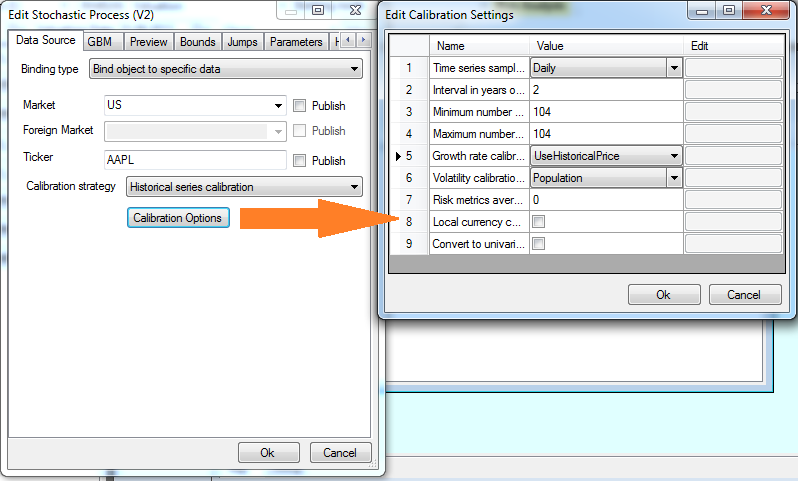
\includegraphics[width=0.7\textwidth]{./Figures/DataSourcesTab.png}
\caption{Data Sources Tab allows to specify how the stochastic process is connected to the market data.}
\label{fig.DataSourceTab}
\end{center}
\end{figure}

\begin{figure}[h]
\begin{center}
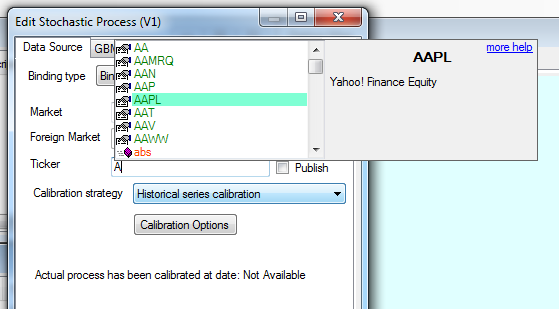
\includegraphics[width=0.7\textwidth]{./Figures/Autocomplete.png}
\caption{By pressing CTRL+SPACE, it's possible to retrieve additional information on tickers and auto-complete them.}
\label{fig.DataSourceTab}
\end{center}
\end{figure}


\begin{figure}[h]
\begin{center}
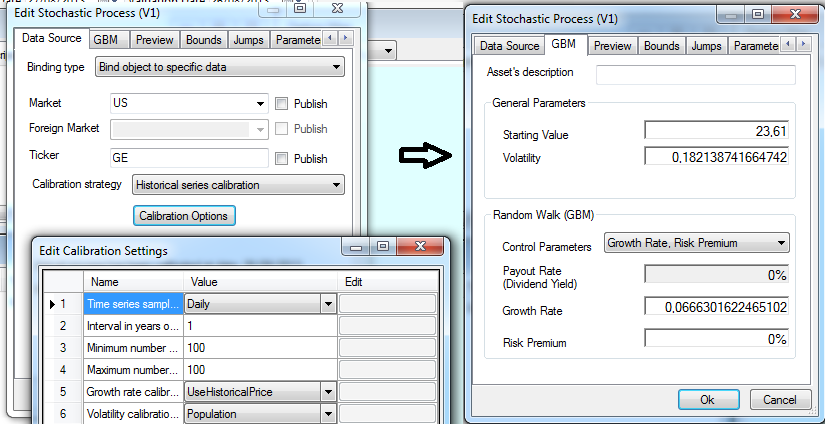
\includegraphics[width=0.7\textwidth]{./Figures/HistoricalCalibration.png}
\caption{Example of calibration of a GBM model to the historical series of General Electric (GE) stock prices.}
\label{fig.DataSourceTab}
\end{center}
\end{figure}


\end{document}


